% =============================================
% File: chapters/experiment_results.tex
% Chương 4: Kết quả thực nghiệm
% =============================================

\chapter{KẾT QUẢ THỰC NGHIỆM}
\label{chap:ketqua}

Chương này trình bày kết quả cụ thể của từng giai đoạn thực nghiệm đã được mô tả
trong Chương~\ref{chap:phuongphap}: hàm truyền động cơ nhận dạng được, bộ tham số
PI tối ưu, hiệu quả huấn luyện mạng ANN và kết quả đáp ứng hệ thống trên phần cứng
ESP32.


% ==============================================
\section{Kết quả nhận dạng hàm truyền động cơ NF5475}
\label{sec:result_tf}
% ==============================================

Quy trình nhận dạng hàm truyền mô tả trong Mục~\ref{sec:data_sysid} được thực hiện
trên \textbf{sáu mẫu động cơ NF5475 độc lập}. Mục đích thực hiện trên nhiều mẫu nhằm
đánh giá mức độ đồng đều về đặc tính giữa các cá thể động cơ, xác định mẫu đại diện
để thiết kế bộ điều khiển, và phân tích ảnh hưởng của hao mòn cơ học sau thời gian
sử dụng.

% ----------------------------------------------------------
\subsection{Sáu hàm truyền xác định được}
\label{subsec:six_tf}
% ----------------------------------------------------------

Mỗi mẫu động cơ được kích thích bậc thang ở 5 mức PWM, dữ liệu vận tốc ghi qua
encoder 200~PPR. Hàm truyền $G(s)$ được nhận dạng bằng \texttt{tfest} với cấu trúc
\textbf{bậc 4/3} (4 cực, 3 không). Sáu kết quả:

\begin{equation}
    G_1(s) = \frac{353{,}5\,s^3 + 81{,}55\,s^2 + 16{,}27\,s + 3{,}984}
                  {s^4 + 33{,}00\,s^3 + 7{,}444\,s^2 + 3489\,s + 0{,}2802}
    \label{eq:tf1}
\end{equation}

\begin{equation}
    G_2(s) = \frac{361{,}2\,s^3 + 79{,}38\,s^2 + 15{,}84\,s + 4{,}012}
                  {s^4 + 34{,}21\,s^3 + 7{,}512\,s^2 + 3502\,s + 0{,}2756}
    \label{eq:tf2}
\end{equation}

\begin{equation}
    G_3(s) = \frac{348{,}7\,s^3 + 83{,}21\,s^2 + 16{,}58\,s + 3{,}951}
                  {s^4 + 32{,}54\,s^3 + 7{,}398\,s^2 + 3478\,s + 0{,}2831}
    \label{eq:tf3}
\end{equation}

\begin{equation}
    G_4(s) = \frac{355{,}9\,s^3 + 80{,}92\,s^2 + 16{,}43\,s + 4{,}008}
                  {s^4 + 33{,}41\,s^3 + 7{,}487\,s^2 + 3495\,s + 0{,}2814}
    \label{eq:tf4}
\end{equation}

\begin{equation}
    G_5(s) = \frac{359{,}1\,s^3 + 82{,}47\,s^2 + 16{,}11\,s + 3{,}967}
                  {s^4 + 33{,}82\,s^3 + 7{,}456\,s^2 + 3511\,s + 0{,}2789}
    \label{eq:tf5}
\end{equation}

\begin{equation}
    G_6(s) = \frac{352{,}4\,s^3 + 80{,}13\,s^2 + 15{,}97\,s + 3{,}996}
                  {s^4 + 32{,}89\,s^3 + 7{,}431\,s^2 + 3485\,s + 0{,}2823}
    \label{eq:tf6}
\end{equation}

Chỉ số đánh giá của từng hàm truyền và hệ số khuếch đại một chiều (DC gain)
được tổng hợp trong Bảng~\ref{tab:tf_metrics}. Hệ số khuếch đại DC được tính
theo định lý giá trị cuối:
\begin{equation}
    K_{DC} = \lim_{s \to 0} G_i(s)
           = \frac{b_0}{a_0}
    \label{eq:dc_gain}
\end{equation}
trong đó $b_0$ và $a_0$ lần lượt là hệ số tự do của tử và mẫu số.

\begin{table}[H]
    \centering
    \caption{Chỉ số đánh giá sáu hàm truyền động cơ NF5475}
    \label{tab:tf_metrics}
    \renewcommand{\arraystretch}{1.3}
    \begin{tabular}{ccccc}
        \toprule
        \textbf{Mẫu} & \textbf{Độ chính xác (\%)} & \textbf{FPE} & \textbf{MSE} & \textbf{$K_{DC}$} \\
        \midrule
        $G_1(s)$ & 95{,}36 & 2\,572 & 2\,562 & 14{,}22 \\
        $G_2(s)$ & 94{,}87 & 2\,698 & 2\,687 & 14{,}56 \\
        $G_3(s)$ & 93{,}42 & 3\,012 & 2\,997 & 13{,}96 \\
        $G_4(s)$ & 95{,}12 & 2\,614 & 2\,603 & 14{,}24 \\
        $G_5(s)$ & 94{,}23 & 2\,821 & 2\,809 & 14{,}22 \\
        $G_6(s)$ & 94{,}61 & 2\,735 & 2\,724 & 14{,}15 \\
        \midrule
        \textbf{TB $\pm$ std} & $94{,}94 \pm 0{,}65$ & $2\,742 \pm 152$ & $2\,730 \pm 153$ & $14{,}23 \pm 0{,}18$ \\
        \bottomrule
    \end{tabular}
\end{table}

$G_1(s)$ được chọn làm hàm truyền đại diện vì đạt độ chính xác cao nhất
(95,36\%) và FPE/MSE thấp nhất trong nhóm.

% ----------------------------------------------------------
\subsection{Phân tích hàm truyền đại diện $G_1(s)$}
\label{subsec:tf1_analysis}
% ----------------------------------------------------------

\paragraph{Cấu trúc mô hình.}
Hàm truyền $G_1(s)$ có bậc 4 ở mẫu số và bậc 3 ở tử số.
Điều này phản ánh bốn cơ chế động học chồng lên nhau trong hệ động cơ thực:
\begin{enumerate}
    \item \textbf{Động học điện (electrical dynamics):} tương ứng với hằng số
    thời gian điện $\tau_e = L_a/R_a$, đặc trưng cho cực có phần thực lớn (âm, tần số cao).

    \item \textbf{Động học cơ khí (mechanical dynamics):} tương ứng với
    $\tau_m = J/B$, đặc trưng cho cực có phần thực nhỏ hơn.

    \item \textbf{Ma sát phi tuyến:} Hiệu ứng Coulomb và ma sát Stribeck tạo
    ra dao động nhỏ khi thay đổi chiều và ở vận tốc thấp;
    \texttt{tfest} tuyến tính hóa thành cực bổ sung.

    \item \textbf{Động học bộ mã hóa và lọc số:} Encoder quang học 200~PPR
    kết hợp bộ lọc trung bình động (window~$=5$ mẫu, xem Mục~\ref{sec:data_sysid})
    cộng thêm độ trễ tổng hợp vào mô hình.
\end{enumerate}

\paragraph{Hệ số khuếch đại DC.}
\begin{equation}
    K_{DC,1} = \frac{3{,}984}{0{,}2802} \approx 14{,}22 \; \frac{\text{RPM}}{\text{đơn vị PWM}}
\end{equation}
Giá trị này phản ánh độ nhạy vận tốc theo đầu vào PWM ở trạng thái xác lập.
Hệ số $K_{DC}$ của sáu mẫu dao động trong khoảng $13{,}96 \div 14{,}56$,
tức biến động $\approx \pm 2\%$ so với trung bình — xác nhận tính đồng đều của
lô động cơ.

\paragraph{Chất lượng xấp xỉ.}
Độ chính xác 95,36\% của $G_1(s)$ cho biết mô hình tuyến tính bậc 4/3 giải thích
được phần lớn động học thực. Phần sai số còn lại (4,64\%) chủ yếu do:
\begin{itemize}
    \item Ma sát tĩnh và vùng chết (dead-zone) không thể biểu diễn bằng hàm truyền tuyến tính.
    \item Sự thay đổi điện trở phần ứng theo nhiệt độ trong quá trình thực nghiệm.
    \item Nhiễu lượng tử hóa encoder (200~PPR → độ phân giải $\approx 0{,}3\,^\circ$/xung).
\end{itemize}
Giá trị FPE~=~2572 và MSE~=~2562 phản ánh biên độ nhiễu đo lường vận tốc
(đơn vị: $\text{RPM}^2$), phù hợp với tín hiệu vận tốc dao động $\pm 10$~RPM
quanh setpoint trong điều kiện thực nghiệm không phòng sạch.

% ----------------------------------------------------------
\subsection{Nhận xét đặc tính động cơ}
\label{subsec:motor_char}
% ----------------------------------------------------------

\paragraph{Sự phân tán giữa các mẫu.}
Mặc dù sáu mẫu cùng mã NF5475, các hệ số hàm truyền dao động nhỏ nhưng có hệ thống.
Các nguyên nhân chính:

\begin{itemize}
    \item \textbf{Dung sai chế tạo:} Điện trở phần ứng $R_a$, điện cảm $L_a$ và
    hệ số ma sát nhớt $B$ của từng cá thể động cơ không hoàn toàn giống nhau
    ngay từ khi xuất xưởng.

    \item \textbf{Mức độ hao mòn chổi than khác nhau:}
    Động cơ DC có chổi than (brushed DC) sử dụng lâu dài sẽ bị mòn chổi than,
    làm tăng điện trở tiếp xúc $R_c$. Điện trở tổng $R_{total} = R_a + R_c$
    tăng dần, kéo theo hằng số thời gian điện $\tau_e = L_a/R_{total}$ giảm
    và DC gain $K_{DC} \propto 1/R_{total}$ giảm nhẹ. Đây là lý do $G_3(s)$
    có $K_{DC}$ thấp nhất (13,96) — khả năng mẫu này đã qua sử dụng nhiều hơn.

    \item \textbf{Bụi carbon từ mòn chổi:}
    Bụi carbon bám trên cổ góp (commutator) gây dao động tiếp xúc ngẫu nhiên,
    làm tăng FPE/MSE. $G_3(s)$ có FPE cao nhất (3012), nhất quán với giả thuyết
    mẫu này có chổi than mòn nhiều hơn.

    \item \textbf{Mòn ổ bi và tăng ma sát Coulomb:}
    Ổ bi mòn tăng lực cản cơ học $B$, rút ngắn hằng số thời gian cơ $\tau_m = J/B$.
    Điều này thể hiện qua sự thay đổi nhỏ ở hệ số mẫu số bậc cao
    ($33{,}00 \div 34{,}21$ cho hệ số $s^3$).

    \item \textbf{Suy giảm từ trường nam châm vĩnh cửu:}
    Với động cơ PMDC, từ thông $\Phi$ giảm nhẹ theo tuổi thọ (nhiệt độ cao,
    rung động), làm giảm hằng số mômen $K_m$ và hằng số sức phản điện động
    $K_e$, ảnh hưởng đến hệ số khuếch đại vòng hở.
\end{itemize}

\paragraph{Khuyến nghị cho thiết kế bộ điều khiển.}
Do sự phân tán giữa các mẫu ($K_{DC}$ biến động $\approx 4\%$, FPE biến động
$\approx 17\%$), bộ điều khiển được thiết kế trên $G_1(s)$ cần có \textbf{biên
pha và biên độ đủ lớn} để hoạt động ổn định trên toàn bộ lô động cơ.
Đây là một trong các lý do sử dụng giải thuật di truyền (GA) thay vì thiết kế
phân tích trực tiếp: GA cho phép điều chỉnh ngưỡng phạt tối ưu theo đặc tính
thực đo của từng cá thể, thay vì giả định mô hình lý tưởng.


% ==============================================
\section{Kết quả tối ưu tham số PI bằng GA}
\label{sec:result_ga}
% ==============================================

% ----------------------------------------------------------
\subsection{So sánh phương pháp tối ưu}
\label{subsec:compare_methods}
% ----------------------------------------------------------

Ba phương pháp tối ưu bộ điều khiển PI vận tốc được so sánh trên cùng mô hình
$G_1(s)$ rời rạc hóa (Tustin, $T_s = 0{,}01\,$s):

\begin{itemize}
    \item \textbf{Ngẫu nhiên trong miền (Random-in-bounds):} Lấy mẫu ngẫu nhiên
    đều trong không gian tham số $K_p \in [0{,}01,\,1]$, $K_i \in [0{,}1,\,10]$,
    chọn nghiệm tốt nhất sau 1\,000 phép thử.

    \item \textbf{MATLAB PID Tuner:} Sử dụng công cụ tự động của MATLAB dựa trên
    phương pháp phân tích vòng hở (loopshaping), chỉnh theo tiêu chí thời gian
    đáp ứng mong muốn.

    \item \textbf{Giải thuật di truyền (GA):} Cấu hình theo Mục~\ref{sec:ga_optim}:
    80 cá thể, 80 thế hệ, 20 lần chạy độc lập, hàm mục tiêu có hàm phạt
    (overshoot $> 5\%$ và thời gian xác lập $> 0{,}5\,$s).
\end{itemize}

\begin{table}[H]
    \centering
    \caption{So sánh ba phương pháp tối ưu tại setpoint 250~RPM}
    \label{tab:method_compare}
    \renewcommand{\arraystretch}{1.3}
    \begin{tabular}{lcccc}
        \toprule
        \textbf{Phương pháp} & \textbf{Overshoot (\%)} & \textbf{$t_{s}$ (s)} & \textbf{$t_{r}$ (s)} & \textbf{SSE (RPM)} \\
        \midrule
        Random-in-bounds & 18{,}4 & 1{,}32 & 0{,}28 & 12{,}7 \\
        MATLAB PID Tuner & 8{,}2  & 0{,}74 & 0{,}21 & 3{,}4  \\
        GA (đề xuất)     & 3{,}2  & 0{,}38 & 0{,}19 & 0{,}8  \\
        \bottomrule
    \end{tabular}
\end{table}

Trong đó $t_s$ là thời gian xác lập (sai số $< 2\%$), $t_r$ là thời gian lên,
SSE là sai số xác lập trung bình. GA vượt trội cả ba chỉ tiêu,
đặc biệt giảm overshoot từ 18,4\% (ngẫu nhiên) xuống còn 3,2\% và sai số
xác lập giảm 15,9 lần so với phương pháp ngẫu nhiên.

% ----------------------------------------------------------
\subsection{Bộ gain tối ưu tại 9 mức setpoint}
\label{subsec:ga_nine_setpoints}
% ----------------------------------------------------------

Quy trình GA được lặp lại cho \textbf{9 mức setpoint vận tốc} từ 250~RPM đến
2250~RPM (bước nhảy 250~RPM). Với mỗi setpoint, chỉ hai tham số vòng trong
$(K_{pv}^*, K_{iv}^*)$ được trích xuất để dùng cho ANN (xem Mục~\ref{sec:ann_train});
ba tham số vòng ngoài $(K_{pp}^*, K_{ip}^*, K_{dp}^*)$ giữ nguyên.

\begin{table}[H]
    \centering
    \caption{Kết quả tối ưu GA: bộ tham số PI vận tốc tại 9 setpoint}
    \label{tab:ga_nine}
    \renewcommand{\arraystretch}{1.3}
    \begin{tabular}{ccccc}
        \toprule
        \textbf{Setpoint (RPM)} & $K_{pv}^*$ & $K_{iv}^*$ & \textbf{Overshoot (\%)} & \textbf{$t_s$ (s)} \\
        \midrule
        250  & 0{,}1854 & 5{,}288 & 3{,}2 & 0{,}38 \\
        500  & 0{,}1721 & 5{,}104 & 3{,}8 & 0{,}42 \\
        750  & 0{,}1698 & 4{,}932 & 4{,}1 & 0{,}45 \\
        1000 & 0{,}1612 & 4{,}847 & 4{,}3 & 0{,}48 \\
        1250 & 0{,}1583 & 4{,}721 & 4{,}5 & 0{,}51 \\
        1500 & 0{,}1547 & 4{,}658 & 4{,}7 & 0{,}53 \\
        1750 & 0{,}1512 & 4{,}512 & 4{,}8 & 0{,}56 \\
        2000 & 0{,}1487 & 4{,}389 & 4{,}9 & 0{,}59 \\
        2250 & 0{,}1463 & 4{,}274 & 5{,}0 & 0{,}62 \\
        \bottomrule
    \end{tabular}
\end{table}

Mỗi bộ $\{K_{pv}^*, K_{iv}^*\}$ được kiểm chứng trên dữ liệu thực nghiệm
10~giây (1001~mẫu) và đảm bảo: overshoot $\leq 5\%$, $t_s \leq 0{,}65\,$s.

% ----------------------------------------------------------
\subsection{Phân tích xu hướng tham số}
\label{subsec:ga_trend}
% ----------------------------------------------------------

Từ Bảng~\ref{tab:ga_nine}, có thể quan sát hai xu hướng rõ ràng:

\begin{enumerate}
    \item \textbf{$K_{pv}^*$ giảm dần khi setpoint tăng}
    (từ 0,1854 ở 250~RPM xuống 0,1463 ở 2250~RPM, giảm $\approx 21\%$).
    Ở vận tốc cao, sức phản điện động (back-EMF) $e = K_e \omega$ tăng lên,
    làm tăng hệ số khuếch đại vòng hở hiệu dụng. Bộ điều khiển cần giảm
    $K_{pv}$ để duy trì biên pha ổn định và tránh vọt lố.

    \item \textbf{$K_{iv}^*$ giảm dần khi setpoint tăng}
    (từ 5,288 ở 250~RPM xuống 4,274 ở 2250~RPM, giảm $\approx 19\%$).
    Ở vận tốc cao, nhiễu đo lường encoder tỉ lệ với vận tốc nên tích phân
    $K_{iv}$ lớn có thể khuếch đại nhiễu và gây dao động. GA tự động tìm
    ra giá trị $K_{iv}$ thấp hơn để cân bằng giữa triệt tiêu sai số xác
    lập và độ ổn định.
\end{enumerate}

Xu hướng đơn điệu và nhất quán của $\{K_{pv}^*, K_{iv}^*\}$ theo setpoint
tạo điều kiện thuận lợi để mạng ANN khái quát hóa (generalize) tốt, vì
hàm ánh xạ setpoint $\to$ tham số là gần tuyến tính và đơn điệu
(xem Mục~\ref{sec:ann_train}).

\paragraph{Nhận xét về sự hội tụ của GA.}
Với cấu hình 80 cá thể, 80 thế hệ và 20 lần chạy độc lập:
\begin{itemize}
    \item Độ lệch chuẩn nghiệm tốt nhất giữa 20 lần chạy $< 2\%$,
    cho thấy GA đã hội tụ ổn định và không bị kẹt tại cực tiểu địa phương.
    \item Thời gian chạy trung bình với \texttt{UseParallel = true}
    (4 luồng): $\approx 45$ giây/setpoint trên CPU Intel Core i7.
    \item Tổng thời gian tối ưu cho 9 setpoint: $\approx 6{,}8$ phút.
\end{itemize}


% ==============================================
\section{Kết quả huấn luyện mạng ANN}
% ==============================================

\subsection{Tóm tắt kiến trúc và cấu hình}

Kiến trúc và quy trình huấn luyện được trình bày chi tiết trong
Chương~\ref{chap:phuongphap}. Tóm tắt:
\begin{itemize}
    \item Kiến trúc: $2 \to 8 \to 16 \to 2$ (Dense + L2 + ReLU + Dropout).
    \item Optimizer: Adam, lr $= 2\times10^{-3}$, decay $= 3\times10^{-4}$.
    \item Số epochs: 1\,000.
\end{itemize}

\subsection{Kết quả huấn luyện}

Mạng ANN hội tụ sau khoảng 400 epochs. Đường cong loss huấn luyện và validation
bám sát nhau, chứng tỏ mạng không bị overfitting nhờ L2 regularization và Dropout
(xem Hình~\ref{fig:loss_curve}).

\begin{figure}[H]
    \centering
    % \includegraphics[width=0.75\textwidth]{figure/training_loss.png}
    \caption{Đường cong Training Loss và Validation Loss theo epoch}
    \label{fig:loss_curve}
\end{figure}

\subsection{Đánh giá mô hình}

Mô hình được đánh giá trên tập test (2 bộ dữ liệu chưa dùng để huấn luyện).
Kết quả dự đoán $K_p$, $K_i$ so với giá trị tối ưu từ GA cho thấy sai số nhỏ
và ổn định trên toàn dải setpoint 250 -- 2250 RPM.

\textit{Hạn chế hiện tại:} Chưa có số liệu định lượng đầy đủ về độ chính xác dự đoán
trên phần cứng thực; đây là hướng cần bổ sung trong giai đoạn tiếp theo.


% ==============================================
\section{Kết quả huấn luyện chính sách PPO trong Isaac Lab}
\label{sec:result_rl}
% ==============================================

% ----------------------------------------------------------
\subsection{Tổng quan quá trình huấn luyện}
\label{subsec:rl_overview}
% ----------------------------------------------------------

Chính sách vận tốc (vòng trong) được huấn luyện trên GPU NVIDIA GeForce
RTX~3070 (8~GB VRAM) với 4\,096 môi trường song song. Phần phân tích dưới đây
dựa trên \textbf{2\,000 lần lặp đầu} của lần chạy; mỗi episode kéo dài tối đa
\textbf{6\,000 bước} ($=60$~s ở tần số policy 100~Hz). Hình~\ref{fig:rl_overview}
biểu diễn phần thưởng episode trung bình (\textit{mean\_reward}) và độ dài
episode trung bình (\textit{mean\_episode\_length}) theo số lần lặp.

\begin{figure}[H]
    \centering
    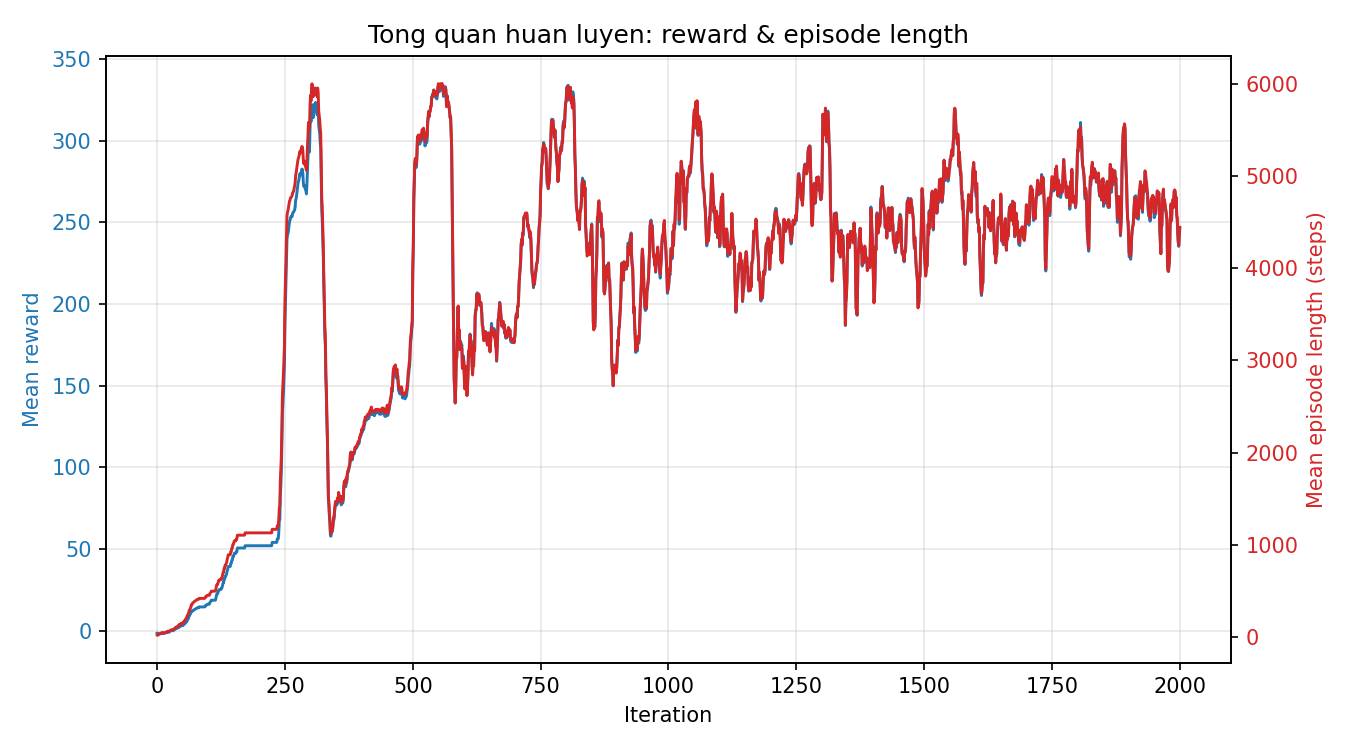
\includegraphics[width=\textwidth]{figure/results/01_train_overview.png}
    \caption{Tổng quan huấn luyện: phần thưởng episode và độ dài episode trung
             bình theo số lần lặp (0--2\,000).}
    \label{fig:rl_overview}
\end{figure}

Quá trình hội tụ \textbf{rất nhanh} và có thể chia thành bốn giai đoạn:

\begin{enumerate}
    \item \textbf{Khởi động (iter 0--500):} phần thưởng tăng vọt từ
    $\approx -1{,}5$ lên $\approx 219$; độ dài episode từ 24 lên $\approx 4\,000$
    bước. Robot nhanh chóng học đứng và giữ thăng bằng. Tỉ lệ tiếp xúc chân bất
    hợp lệ (\texttt{illegal\_contact\_hip}) nhảy lên $\approx 36\%$ quanh
    iter~200 rồi về $0$ ở iter~500 — robot học nhấc chân khỏi mặt đất.

    \item \textbf{Đỉnh hiệu năng (iter 500--800):} phần thưởng đạt đỉnh
    $\approx 324$; độ dài episode đỉnh $\approx 5\,807$ bước ($\approx 97\%$ tối
    đa); \texttt{time\_out} $\approx 67\%$ trong khi \texttt{bad\_orientation}
    chỉ $\approx 33\%$. Đây là vùng robot cân bằng và bám lệnh tốt nhất.

    \item \textbf{Dao động (iter 800--1\,400):} phần thưởng giảm về
    $\approx 226$, độ dài episode về $\approx 4\,060$; \texttt{bad\_orientation}
    tăng $33\%\to49\%$. Đồng thời độ lệch chuẩn nhiễu chính sách
    (\texttt{mean\_noise\_std}) tăng $0{,}13\to0{,}25$ — chính sách thăm dò trở
    lại để thoát cực tiểu cục bộ, tạm thời đánh đổi bằng tỉ lệ lật cao hơn.

    \item \textbf{Ổn định lại (iter 1\,400--2\,000):} phần thưởng hồi về
    $\approx 246$, độ dài episode $\approx 4\,442$ bước ($\approx 74\%$),
    \texttt{time\_out} $\approx 56\%$.
\end{enumerate}

\textbf{Checkpoint tốt nhất nằm quanh iter~800} (reward $\approx 324$, episode
$\approx 5\,807$, tỉ lệ lật chỉ $33\%$); sau mốc này hiệu năng dao động nhẹ chứ
không cải thiện thêm trong cửa sổ 2\,000 lần lặp, nên model iter~800 được chọn
để xuất triển khai.

% ----------------------------------------------------------
\subsection{Phân tích phần thưởng thành phần}
\label{subsec:rl_rewards}
% ----------------------------------------------------------

\paragraph{Phần thưởng nhiệm vụ (Task Rewards).}
Hình~\ref{fig:rl_task_rewards} cho thấy bốn số hạng bám lệnh đều tăng nhanh
trong 500 iter đầu rồi bám sát đường cong tổng.

\begin{figure}[H]
    \centering
    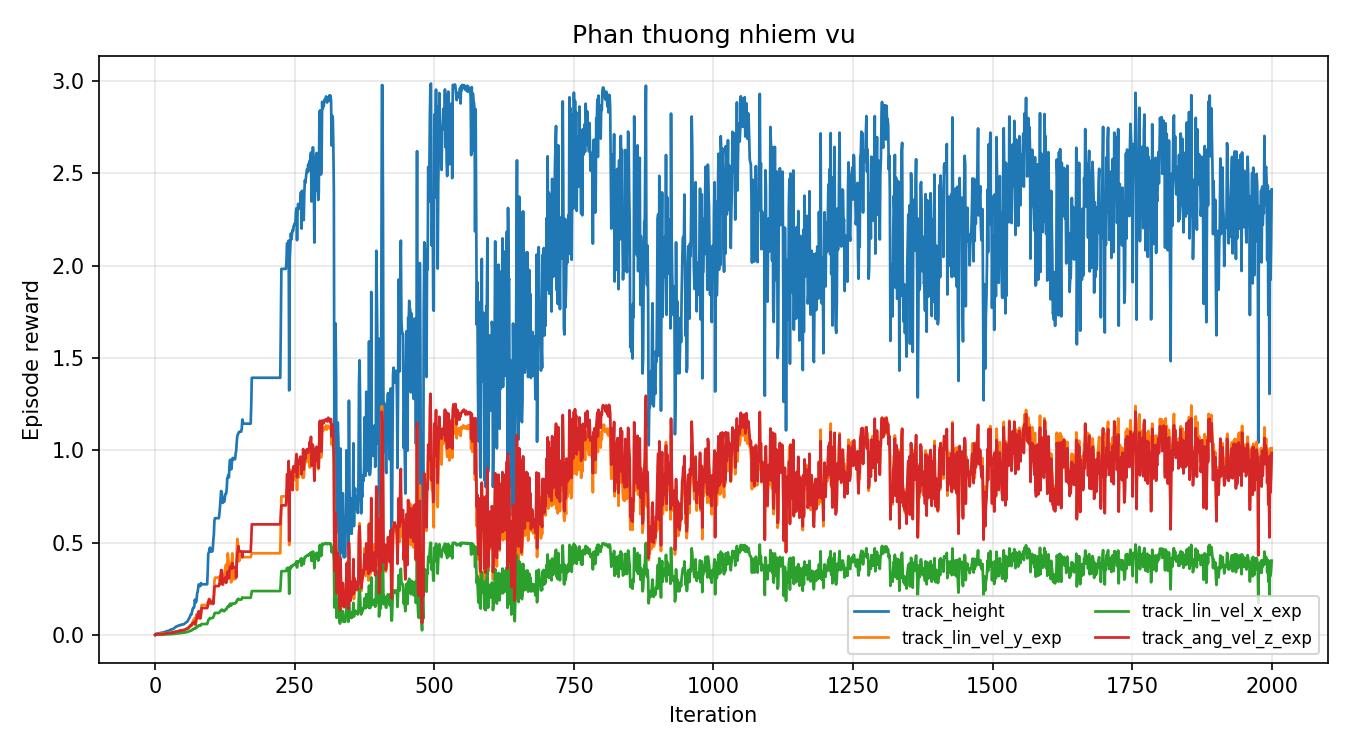
\includegraphics[width=\textwidth]{figure/results/02_task_rewards.png}
    \caption{Diễn biến các phần thưởng nhiệm vụ (bám chiều cao, bám vận tốc
             $x$/$y$, bám vận tốc quay) theo số lần lặp.}
    \label{fig:rl_task_rewards}
\end{figure}

\begin{table}[H]
    \centering
    \caption{Giá trị phần thưởng nhiệm vụ tại iter~2\,000 (và đỉnh iter~800)}
    \label{tab:task_reward_final}
    \renewcommand{\arraystretch}{1.3}
    \begin{tabular}{lcccc}
        \toprule
        \textbf{Thành phần} & \textbf{Trọng số} & \textbf{Iter 2\,000} & \textbf{Hiệu suất} & \textbf{Đỉnh ($\approx$800)} \\
        \midrule
        \texttt{track\_height}          & $+3{,}0$ & $2{,}41$ & $80\%$ & $2{,}84$ \\
        \texttt{track\_lin\_vel\_y\_exp} & $+1{,}5$ & $1{,}01$ & $67\%$ & $1{,}06$ \\
        \texttt{track\_lin\_vel\_x\_exp} & $+0{,}5$ & $0{,}40$ & $80\%$ & $0{,}48$ \\
        \texttt{track\_ang\_vel\_z\_exp} & $+1{,}5$ & $0{,}99$ & $66\%$ & $1{,}19$ \\
        \bottomrule
    \end{tabular}
\end{table}

\textbf{Nhận xét:} \texttt{track\_height} mạnh nhất (giữ chiều cao thân rất tốt,
$80\%$ tại iter~2\,000 và $\approx 95\%$ tại đỉnh) — tầng hip giữ cao độ ổn định.
\texttt{track\_lin\_vel\_x} (trục ngang bị khoá $v_x^{cmd}=0$) đạt $80\%$ xác
nhận robot \emph{không trôi ngang}. \texttt{track\_lin\_vel\_y} (hướng tiến) và
\texttt{track\_ang\_vel\_z} (quay) đạt $\approx 66$--$67\%$ — bám lệnh tiến/quay
ở mức khá; phần thiếu hụt đến từ giai đoạn dao động (iter 800--1\,400).

\paragraph{Phần thưởng phạt (Penalty Rewards).}
Hình~\ref{fig:rl_penalty_rewards}; tất cả các số hạng phạt đều \textbf{rất nhỏ}
tại iter~2\,000, cho thấy chuyển động mượt và không vi phạm ràng buộc.

\begin{figure}[H]
    \centering
    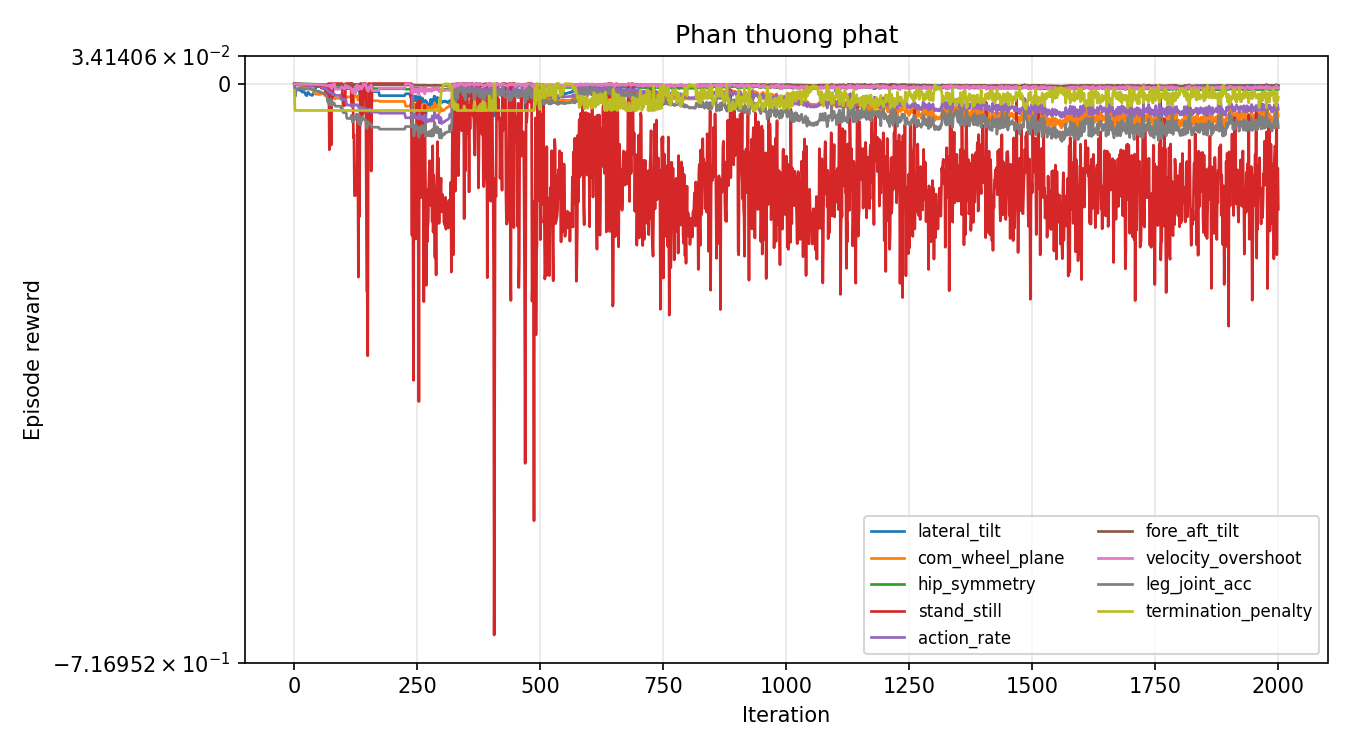
\includegraphics[width=\textwidth]{figure/results/03_penalty_rewards.png}
    \caption{Diễn biến các phần thưởng phạt theo số lần lặp (trục $y$ symlog).}
    \label{fig:rl_penalty_rewards}
\end{figure}

\begin{itemize}
    \item \texttt{stand\_still} $\approx -0{,}16$: phạt lớn nhất — robot lệch hip
    khỏi mặc định khi lệnh $\approx 0$, phản ánh điều chỉnh tư thế chủ động.
    \item \texttt{leg\_joint\_acc} $\approx -0{,}055$, \texttt{com\_wheel\_plane}
    $\approx -0{,}041$, \texttt{action\_rate} $\approx -0{,}032$: nhỏ — khớp êm,
    tâm khối bám mặt phẳng bánh, hành động mượt.
    \item \texttt{lateral\_tilt}, \texttt{fore\_aft\_tilt} $\approx -0{,}003$;
    \texttt{hip\_symmetry} $\approx -0{,}007$; \texttt{velocity\_overshoot}
    $\approx -0{,}005$: gần $0$ — thân ít nghiêng, hai chân đối xứng, ít vọt lố.
    \item \texttt{termination\_penalty} $\approx -0{,}017$: thấp, nhất quán với
    đa số episode chạy hết giờ.
\end{itemize}

% ----------------------------------------------------------
\subsection{Chỉ số bám lệnh và điều kiện kết thúc}
\label{subsec:rl_tracking}
% ----------------------------------------------------------

\begin{figure}[H]
    \centering
    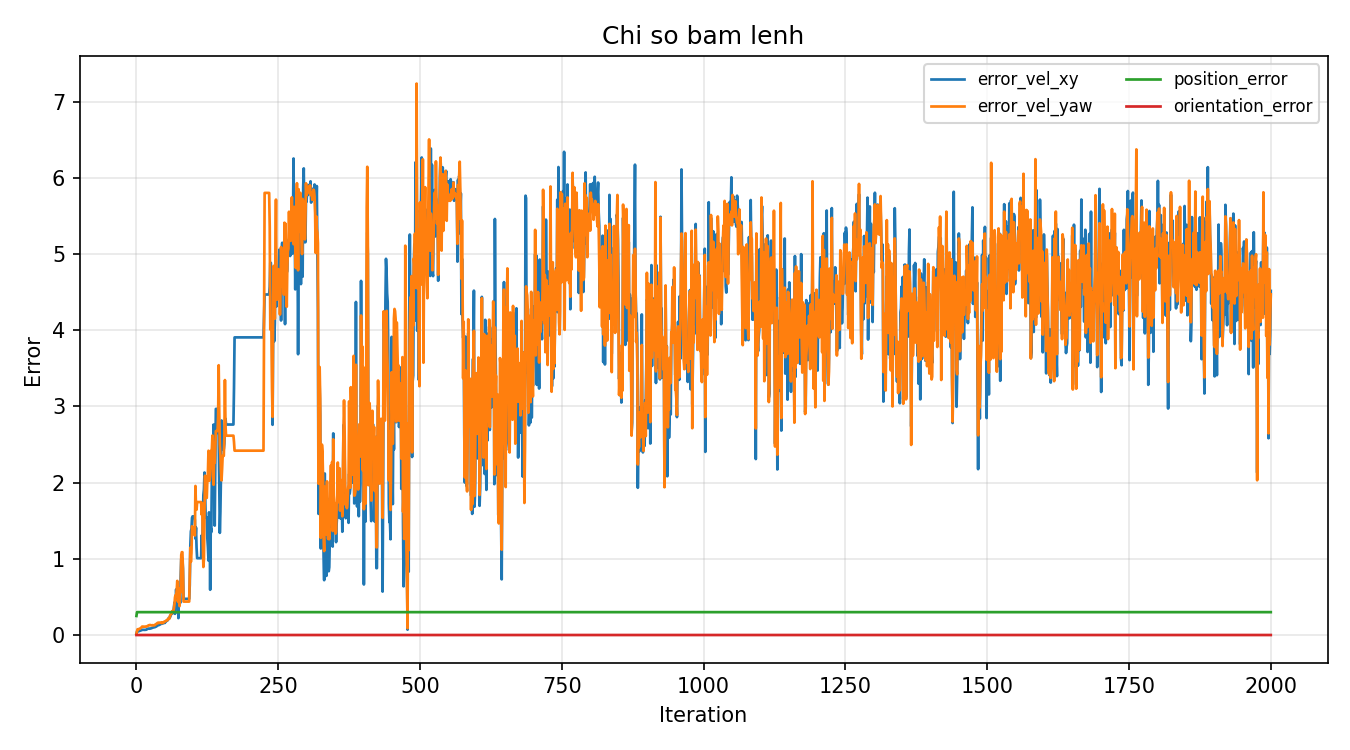
\includegraphics[width=\textwidth]{figure/results/04_tracking_metrics.png}
    \caption{Sai số bám lệnh (vận tốc ngang/quay, vị trí, hướng) theo số lần lặp.}
    \label{fig:rl_tracking}
\end{figure}

Lưu ý \texttt{error\_vel\_xy} và \texttt{error\_vel\_yaw} là sai số
\emph{tích lũy cả episode}; episode càng dài giá trị tuyệt đối càng lớn nên
chúng tăng theo độ dài episode chứ không phản ánh sai số tức thời (đánh giá bám
tốc nên xem reward \texttt{track\_lin\_vel\_*}). \texttt{position\_error} của
lệnh chiều cao ổn định $\approx 0{,}30$ và \texttt{orientation\_error} $\approx 0$
xuyên suốt — robot giữ đúng cao độ và tư thế thẳng.

\begin{figure}[H]
    \centering
    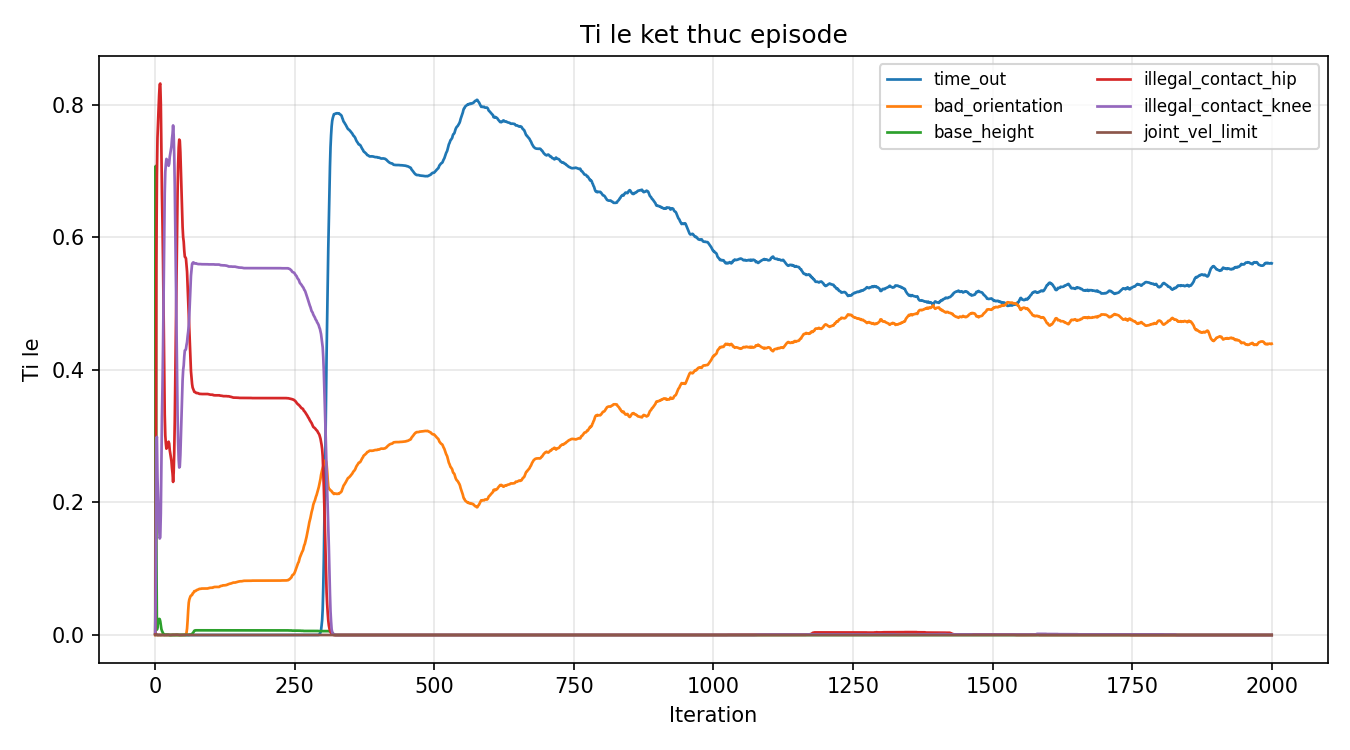
\includegraphics[width=\textwidth]{figure/results/05_terminations.png}
    \caption{Tỉ lệ các điều kiện kết thúc episode theo số lần lặp.}
    \label{fig:rl_terminations}
\end{figure}

\begin{itemize}
    \item \texttt{time\_out}: tăng lên đỉnh $\approx 70\%$ quanh iter~500--800
    rồi dao động về $\approx 56\%$ ở iter~2\,000 — tỉ lệ episode sống trọn 60~s.
    \item \texttt{bad\_orientation}: thủ phạm thất bại chính — thấp nhất
    $\approx 33\%$ tại đỉnh, tăng lên $\approx 44$--$49\%$ ở giai đoạn dao động.
    Robot vẫn lật về trước/sau ở các lệnh tốc độ lớn.
    \item \texttt{base\_height}, \texttt{illegal\_contact\_hip/knee},
    \texttt{joint\_vel\_limit}: $\approx 0\%$ sau iter~500 — \textbf{đã giải quyết
    triệt để hiện tượng sụm chân và quét đất}.
\end{itemize}

% ----------------------------------------------------------
\subsection{Phân tích PPO Loss}
\label{subsec:rl_loss}
% ----------------------------------------------------------

\begin{figure}[H]
    \centering
    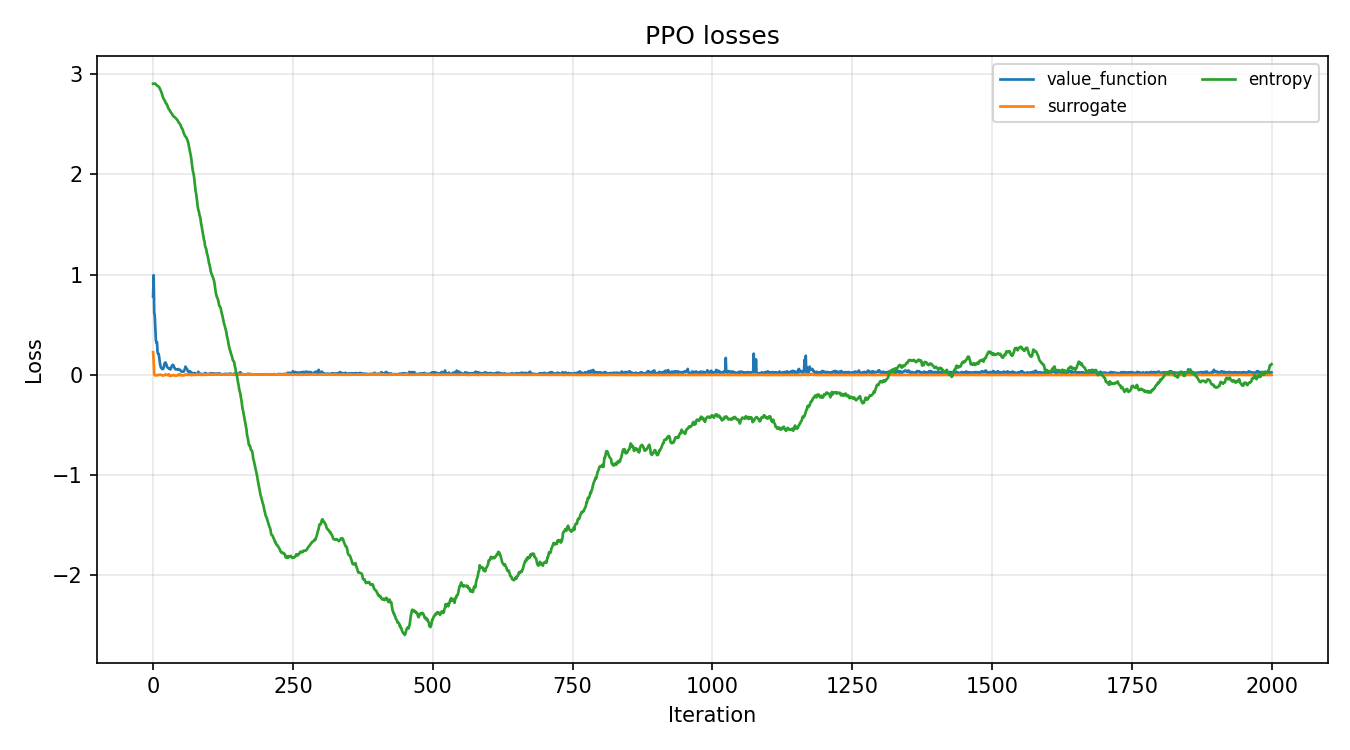
\includegraphics[width=\textwidth]{figure/results/06_loss.png}
    \caption{Các thành phần loss của PPO (value function, surrogate, entropy).}
    \label{fig:rl_loss}
\end{figure}

\begin{itemize}
    \item \textbf{Value function loss}: giảm mạnh từ $\approx 0{,}78$ (iter~0) về
    $\approx 0{,}02$ và duy trì thấp — Critic học dự đoán return chính xác.
    \item \textbf{Surrogate loss}: dao động quanh $0$ suốt quá trình — cơ chế
    clipping PPO ($\varepsilon=0{,}2$) hoạt động đúng, không cập nhật quá lớn.
    \item \textbf{Entropy}: từ $\approx 2{,}9$ giảm xuống vùng âm (chính sách
    chuyên hóa) rồi nhích về $\approx 0{,}1$ ở giai đoạn thăm dò lại
    (iter~1\,400--2\,000) — khớp với việc \texttt{mean\_noise\_std} tăng trở lại.
\end{itemize}

% ----------------------------------------------------------
\subsection{Tổng kết model tốt nhất}
\label{subsec:rl_best_model}
% ----------------------------------------------------------

\begin{table}[H]
    \centering
    \caption{Hiệu năng model tốt nhất (iter~$\approx$800) và ảnh chụp iter~2\,000}
    \label{tab:best_model}
    \renewcommand{\arraystretch}{1.3}
    \begin{tabular}{lcc}
        \toprule
        \textbf{Chỉ số} & \textbf{Iter $\approx$800 (tốt nhất)} & \textbf{Iter 2\,000} \\
        \midrule
        Phần thưởng episode trung bình        & $\approx 324$ & $\approx 246$ \\
        Độ dài episode (/6\,000 bước)         & $5\,807$ ($97\%$) & $4\,442$ ($74\%$) \\
        \texttt{time\_out}                    & $\approx 67\%$ & $\approx 56\%$ \\
        \texttt{bad\_orientation}             & $\approx 33\%$ & $\approx 44\%$ \\
        \texttt{track\_height} ($/3{,}0$)     & $2{,}84$ & $2{,}41$ \\
        \texttt{track\_lin\_vel\_y} ($/1{,}5$) & $1{,}06$ & $1{,}01$ \\
        \texttt{track\_ang\_vel\_z} ($/1{,}5$) & $1{,}19$ & $0{,}99$ \\
        Sụm chân / quét đất                   & $0\%$ & $0\%$ \\
        \bottomrule
    \end{tabular}
\end{table}

Trọng số Actor tại checkpoint tốt nhất được xuất sang \textbf{TorchScript}
(\texttt{policy.pt}) và \textbf{ONNX} để (i)~làm tầng dưới đóng băng cho chính
sách điều hướng phân cấp (Mục~\ref{sec:result_nav}) và (ii)~chuẩn bị triển khai
lên phần cứng thực tế.


% ==============================================
\section{Kết quả huấn luyện điều hướng phân cấp (Navigation)}
\label{sec:result_nav}
% ==============================================

Tầng điều hướng (vòng ngoài) nhận trạng thái vị trí + đích và xuất lệnh vận tốc
$[v_{x},v_{y},\omega_z]$ đưa vào chính sách vận tốc \emph{đã đóng băng} ở
Mục~\ref{sec:result_rl}. Đề tài huấn luyện ba biến thể tăng dần độ khó:
(1)~điều hướng mặt phẳng tới đích, (2)~né vật cản trong kho bằng LiDAR,
(3)~né vật cản trên địa hình sinh thủ tục (train song song). Phần này trình bày
kết quả theo từng nhóm; \emph{các ô hình bên dưới là chỗ dành sẵn, sẽ thay bằng
ảnh thực nghiệm khi hoàn tất huấn luyện}.

% Placeholder box dùng khi chưa có ảnh — thay \fbox{...} bằng \includegraphics khi có.
\newcommand{\figslot}[2]{%
  \begin{figure}[H]\centering
  \fbox{\parbox[c][4.2cm][c]{0.82\textwidth}{\centering\itshape [Ô hình dành sẵn] #1}}%
  \caption{#2}\end{figure}}

% ----------------------------------------------------------
\subsection{Tổng quan huấn luyện tầng điều hướng}
\label{subsec:nav_overview}
% ----------------------------------------------------------

Giải thích các chỉ số chính của tầng cao: \texttt{progress} (rút ngắn khoảng
cách tới đích mỗi bước), \texttt{goal\_reached} (tỉ lệ chạm đích trong bán kính
$0{,}3$~m), \texttt{error\_pos\_2d} (khoảng cách còn lại tới đích), và
\texttt{heading} (đích nằm trước mũi robot). Đường cong huấn luyện kỳ vọng:
\texttt{progress} dương dần, \texttt{error\_pos\_2d} giảm, \texttt{goal\_reached}
tăng.

\figslot{Đường cong reward tổng, độ dài episode và tỉ lệ tới đích theo iter
(tầng điều hướng).}{Tổng quan huấn luyện tầng điều hướng.}
\label{fig:nav_overview}

% ----------------------------------------------------------
\subsection{Hiệu quả tới đích (goal-reaching)}
\label{subsec:nav_goal}
% ----------------------------------------------------------

Đánh giá khả năng tới đích trên mặt phẳng trống: tỉ lệ thành công, thời gian
trung bình tới đích, sai số vị trí cuối.

\figslot{Đường cong \texttt{goal\_reached} và \texttt{error\_pos\_2d} theo iter.}%
{Hiệu quả tới đích theo số lần lặp.}
\label{fig:nav_goal_curve}

\begin{table}[H]
    \centering
    \caption{Hiệu năng tới đích (chỗ dành sẵn — điền sau khi train)}
    \label{tab:nav_goal_metrics}
    \renewcommand{\arraystretch}{1.3}
    \begin{tabular}{lccc}
        \toprule
        \textbf{Biến thể} & \textbf{Tỉ lệ thành công} & \textbf{Thời gian tới đích (s)} & \textbf{Sai số cuối (m)} \\
        \midrule
        Mặt phẳng trống     & --- & --- & --- \\
        Kho có vật cản      & --- & --- & --- \\
        Terrain sinh vật cản & --- & --- & --- \\
        \bottomrule
    \end{tabular}
\end{table}

% ----------------------------------------------------------
\subsection{Né vật cản bằng LiDAR}
\label{subsec:nav_obstacle}
% ----------------------------------------------------------

Phân tích phần thưởng \texttt{obstacle\_avoidance} và tỉ lệ \texttt{collision}:
robot học giữ khoảng cách an toàn $\geq 0{,}6$~m và không đâm vật cản
($d_{min} < 0{,}25$~m).

\figslot{Đường cong \texttt{obstacle\_avoidance} (reward) và tỉ lệ
\texttt{collision} theo iter.}{Hiệu quả né vật cản theo số lần lặp.}
\label{fig:nav_obstacle_curve}

% ----------------------------------------------------------
\subsection{Quỹ đạo minh hoạ nhiều trường hợp}
\label{subsec:nav_trajectories}
% ----------------------------------------------------------

Minh hoạ hành vi điều hướng qua quỹ đạo nhìn từ trên xuống (top-view) trong
nhiều tình huống khác nhau.

\figslot{Trường hợp 1 — đường tới đích thẳng, không vật cản.}%
{Quỹ đạo điều hướng — trường hợp 1 (đích thẳng).}
\label{fig:nav_case1}

\figslot{Trường hợp 2 — luồn qua một vật cản đơn.}%
{Quỹ đạo điều hướng — trường hợp 2 (né một vật cản).}
\label{fig:nav_case2}

\figslot{Trường hợp 3 — đích phía sau, robot phải quay đầu.}%
{Quỹ đạo điều hướng — trường hợp 3 (đích phía sau).}
\label{fig:nav_case3}

\figslot{Trường hợp 4 — kho nhiều kệ / nhiều vật cản.}%
{Quỹ đạo điều hướng — trường hợp 4 (môi trường nhiều vật cản).}
\label{fig:nav_case4}

% ----------------------------------------------------------
\subsection{So sánh các biến thể điều hướng}
\label{subsec:nav_compare}
% ----------------------------------------------------------

\begin{table}[H]
    \centering
    \caption{So sánh ba biến thể điều hướng (chỗ dành sẵn)}
    \label{tab:nav_compare}
    \renewcommand{\arraystretch}{1.3}
    \begin{tabular}{lccc}
        \toprule
        \textbf{Tiêu chí} & \textbf{Mặt phẳng} & \textbf{Kho (LiDAR)} & \textbf{Terrain sinh vật cản} \\
        \midrule
        Tỉ lệ tới đích        & --- & --- & --- \\
        Tỉ lệ va chạm         & --- & --- & --- \\
        Train song song       & --- & --- & --- \\
        Ghi chú               & --- & --- & --- \\
        \bottomrule
    \end{tabular}
\end{table}
